\section{Results and Discussion}
\label{sec:results}
% OWNED BY THE RESULTS AUTHOR: this section is a skeleton. Do not invent numbers; every \maybeinput table is generated by the code.
\subsection{Fine-tuning: training curves and validation}
\begin{figure}[t]\centering
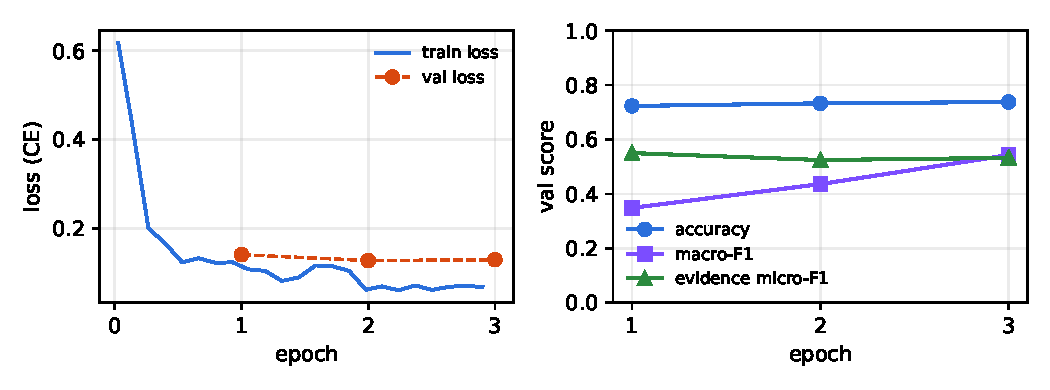
\includegraphics[width=\columnwidth]{figures/training_curves_shared.pdf}
\caption{Logged curves of the shared training run that produced the adapter (joint session, disclosed). Left: training loss per logged optimizer step and validation loss per epoch. Right: per-epoch validation scores computed by that run's own evaluation code, used to select epoch~3. Our independent evaluation is in Table~\ref{tab:cls}.}\label{fig:train}
\end{figure}
Fig.~\ref{fig:train} shows the run that produced the adapter. Its configuration is identical to our \texttt{configs/train.yaml}, and its logs are kept unmodified, with their source, in \texttt{results/finetune/shared\_run/}. The completion-only loss drops from 0.62 to about 0.12 within the first half epoch, then flattens near 0.06--0.07. Validation loss is lowest after epoch~2 (0.127) and almost unchanged after epoch~3 (0.129), so there is no sign of strong overfitting over three epochs on 602 examples. The run selected epoch~3 by validation macro-F1, which keeps rising (0.35, 0.44, 0.54) while accuracy is nearly flat (0.72--0.74). That pattern means the later epochs mainly improve the rare classes. These per-epoch numbers come from the training run's own evaluation and are \emph{not} our results. Our own code (\texttt{configs/train.yaml}, \texttt{src/kormat/finetune/train.py}) reproduces the configuration and was verified end to end only by a CPU smoke run on Qwen2.5-0.5B (loss 0.52$\rightarrow$0.12 over 30 steps, adapter saved and reloaded; \texttt{results/finetune/smoke/}).
\maybeinput{tables/finetune_summary}

\subsection{Before/after on identical examples}
\maybeinput{tables/eval_before_after}
% TODO-INTERPRET: accuracy and macro-F1 change, per-class changes, inclusion vs exclusion, INVALID rate before/after.

\subsection{Evidence retrieval}
\maybeinput{tables/evidence_prf}
% TODO-INTERPRET: P/R/F1, treatment of empty-gold records.

\subsection{Error analysis}
\maybeinput{tables/error_cases}
On the test split the fine-tuned model made 55 label errors out of 206. Another 33 criteria had the right label but a different evidence set: in 19 the model cited sentences outside the expert set, in 17 it missed expert sentences, and some did both. No output was unparsable, and no cited ID was outside the note. Table~\ref{tab:errors} traces eleven distinct cases; the full list with sentence text is in \texttt{docs/research/error\_analysis.md}. Four patterns emerge.

\textbf{(A) Absence treated as proof (28 errors).} \emph{Every} exclusion criterion whose expert label is ``not enough information'' was predicted ``not excluded''. When no sentence mentions the excluding condition (e.g.\ eGFR, prior axillary surgery), the model concludes the patient is not excluded, which is exactly the inference the task forbids. The training data explain the shortcut: 292 of the 388 training exclusion criteria are ``not excluded'', 218 of them without any evidence sentence, against only 65 ``not enough information''. \textbf{(B)} Nine ``not applicable'' exclusions collapse to the same default. Together, A and B make up 37 of the 55 errors and drive exclusion macro-F1 down. For a screening aid this is the unsafe direction, because missing information is hidden rather than flagged.

\textbf{(C) Over-abstention on inferable facts (14).} The opposite failure appears on inclusion criteria that need clinical inference: blood pressure 80/60 with tachycardia means shock (case 185), and an acute femoral complication rules out an elective endarterectomy (161). Case 162 is \emph{contradictory}: the note describes a different vascular problem than the criterion. In several of these cases the model cites the right sentences but abstains. Its evidence localisation is therefore better than its judgement, so the explanation still directs the reviewer to the relevant text. Case 196 is a plain \emph{missing-information} false alarm: the age is stated, but the model misses it. \textbf{(D)} Four errors confuse ``not applicable'' with ``not enough information'' on conditional, sex-specific criteria, where expert conventions themselves vary (case 322).

\textbf{Implication.} A cheap deterministic guard, downgrading an exclusion ``not excluded'' with \emph{empty} evidence to ``not enough information'', would target pattern A without retraining. Rebalancing the exclusion labels during training is the principled fix. We did not apply either to the reported numbers.

\subsection{KV cache}
\maybeinput{tables/kvcache}
\begin{figure}[t]\centering
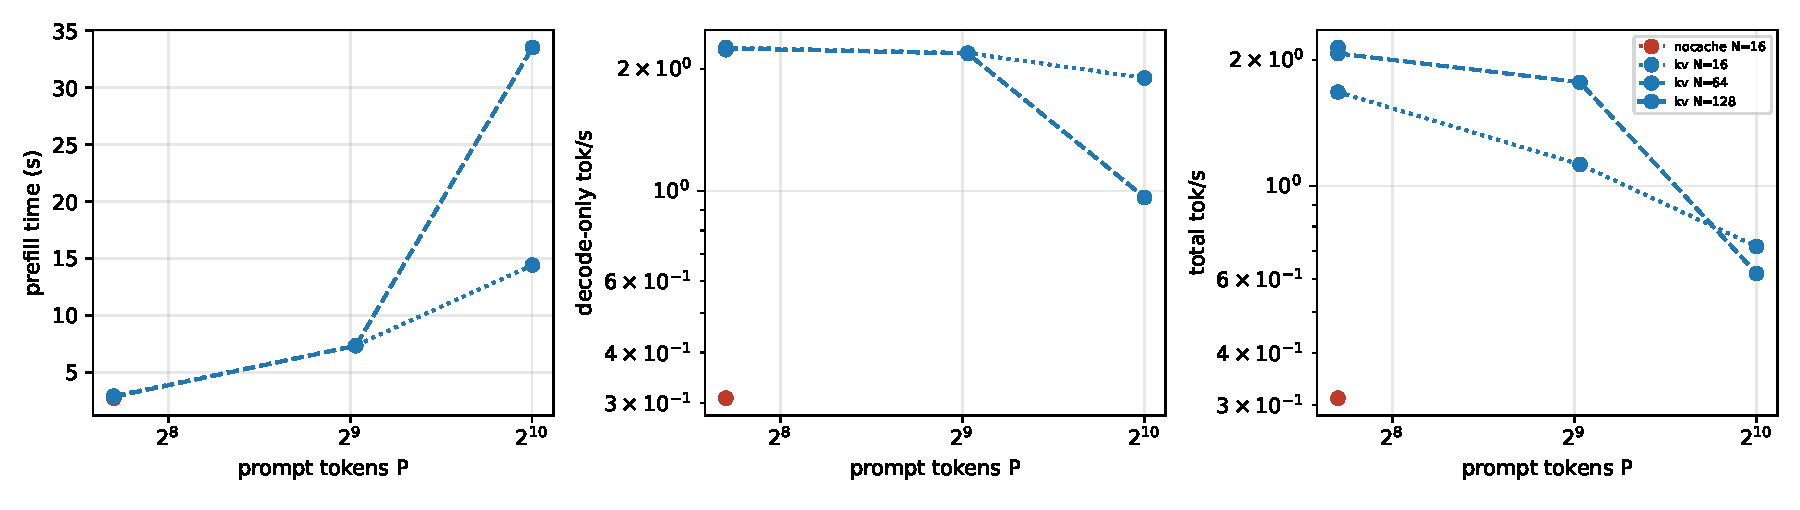
\includegraphics[width=\columnwidth]{figures/kv_speed.pdf}
\caption{Decode throughput of the merged fine-tuned 1.5B model on the CPU, with our pre-allocated KV cache and with the no-cache reference, as a function of prompt length (median of 3 timed runs after 1 warm-up).}\label{fig:kvspeed}
\end{figure}
\textbf{Correctness.} Table~\ref{tab:kveq} shows that the cache-aware decoder reproduces the uncached reference token for token in all five tested input/output combinations ($P\in\{208,523,1025\}$ prompt tokens, $N$ up to 128 new tokens) in fp32. The first-step logits are bit-identical ($\Delta=0$), because both paths run the same prefill. Later steps differ by at most $1.2\times10^{-4}$, which comes from the different reduction order of a $1\times d$ versus a $(P{+}t)\times d$ matrix product, and is far below the top-1/top-2 margin, so no argmax flipped. Our own \texttt{Cache} subclass is provably on the path: a unit test counts its \texttt{update()} calls, and deliberately shifting the position ids breaks equivalence, so the test is not vacuous.

\textbf{Speed.} Table~\ref{tab:kv} and Fig.~\ref{fig:kvspeed} show the asymptotic difference. Without a cache, every new token re-encodes the whole sequence, so decode throughput falls with prompt length (0.31, 0.13 and 0.07 tok/s at $P=208$, 523 and 1025). With the cache, each step processes one token against stored keys and values, and throughput stays roughly flat (2.26, 2.19 and 1.90 tok/s). The measured speed-up therefore grows from $7\times$ to about $17\times$ and $27\times$; the last two compare per-token decode rates measured at different $N$, because the no-cache grid was capped at small $N$ to fit the time budget. Prefill time is the same in both modes (about 2.9\,s at $P=208$), since it is a single forward pass either way.

\textbf{Memory.} Thanks to grouped-query attention (2 KV heads), the analytical cache is only 28\,KB per token in fp32 (12--60\,MB here). That is negligible next to the 6.3\,GB of fp32 weights, so peak RSS barely moves (6.35 to 6.54\,GB). On this hardware the cache trades a few megabytes for an order-of-magnitude speed-up. One outlier ($P=1025$, $N=64$: 0.97 tok/s) was measured while other jobs shared the CPU and is treated as noise.

\textbf{Prefix reuse in evaluation.} The evaluation runner applies the same mechanism across criteria. The system prompt and patient note (273 tokens in the checked example) are prefilled once per patient, and the cache is copied for each criterion. Outputs were token-identical to plain generation (3/3, Table~\ref{tab:prefix}). Per-criterion latency fell from 10.7\,s to 7.2\,s when the prefix was reused, but the mean gain was only about $1.2\times$, because decoding the roughly 15-token answer, not the prompt, dominates on a CPU.
\maybeinput{tables/prefix_cache}

\subsection{Tiled attention}
\maybeinput{tables/attention}
\begin{figure}[t]\centering
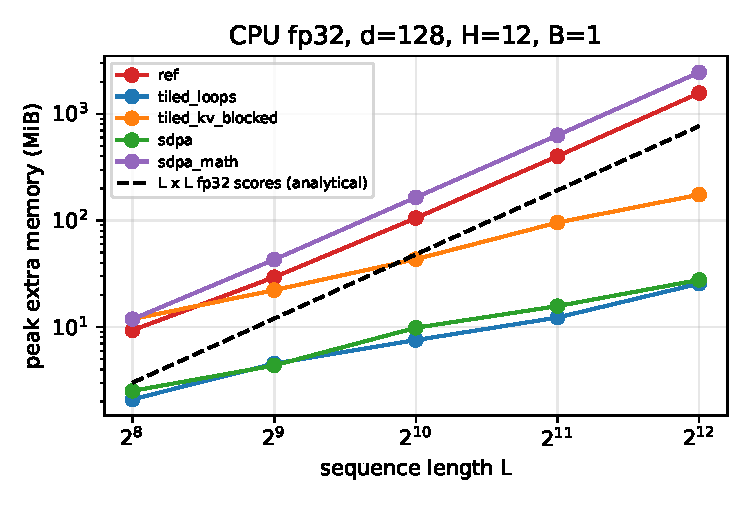
\includegraphics[width=\columnwidth]{figures/attn_memory_vs_L.pdf}
\caption{Peak extra memory of one attention call versus sequence length ($d=128$, 12 heads, fp32, CPU). The reference and the math backend materialise the $L\times L$ score matrix; tiled attention does not.}\label{fig:attnmem}
\end{figure}
\textbf{Correctness.} Across 1{,}680 validation cases (lengths 1 to 1024 including non-multiples of the block size, $L_q\neq L_k$ decode and verify shapes, GQA, causal, padding and fully masked rows, and four block sizes), the tiled online-softmax kernel matches a float64 ground truth within the stated tolerances in every case (Table~\ref{tab:attnval}; timings in Table~\ref{tab:attnbench}). The maximum absolute error is $2.5\times10^{-6}$ in fp32, $9.7\times10^{-4}$ in fp16 and $7.8\times10^{-3}$ in bf16; bf16 needs a relative tolerance of $8\times10^{-3}$ because its unit round-off is $2^{-8}$. A stability test multiplies the logits by 1000: a naive softmax returns NaN, while the running-max formulation stays finite. Routing the attention of a small Qwen2 model through our kernel gives identical greedy tokens (max logit difference about $2\times10^{-7}$).

\textbf{Speed and memory.} The memory advantage is real but the speed advantage is not (Fig.~\ref{fig:attnmem}). At $L=4096$, the reference needs 1.57\,GB of extra memory, close to the 0.77\,GB analytical size of the fp32 score matrix plus the softmax copy, whereas the loop-tiled version needs 26\,MB. Its run time, however, is 5.0\,s against 3.0\,s for the reference and 1.9\,s for PyTorch's fused CPU kernel. This is expected for educational PyTorch code. Each tile launches several separate operators (matmul, max, exp, sum, rescale), each reading and writing main memory. Nothing is fused, and Python loop overhead grows with the number of tiles: run time falls from 8.0\,s at block 16 to 0.6\,s at block 256 for $L=2048$. FlashAttention's speed comes from keeping tiles in on-chip SRAM inside one fused kernel, which plain PyTorch cannot express. On this CPU, therefore, tiling buys linear memory, not speed.

\subsection{Speculative decoding}
\maybeinput{tables/speculative}
\begin{figure}[t]\centering
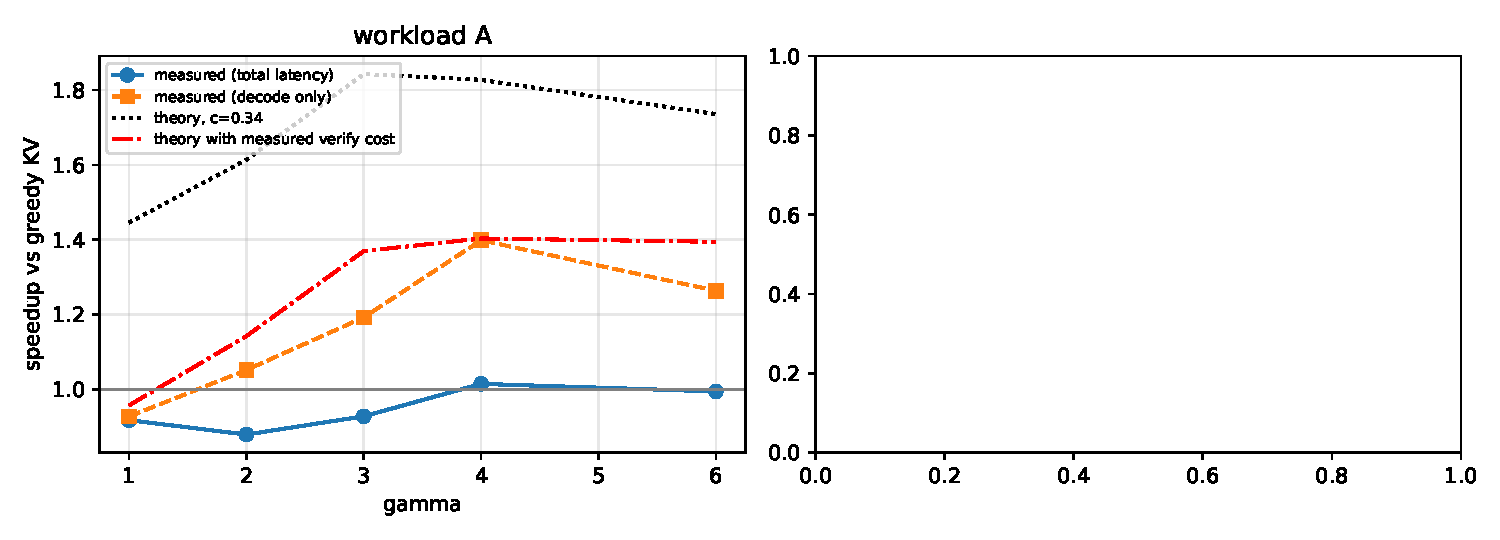
\includegraphics[width=\columnwidth]{figures/spec_speedup.pdf}
\caption{Measured speculative speed-up versus draft length $\gamma$, against the theoretical curve with the measured draft/target cost ratio $c=0.337$, and with the measured verification cost.}\label{fig:spec}
\end{figure}
\textbf{Correctness.} Our draft--verify--rollback decoder produced exactly the target's greedy sequence in 18 of 18 runs on validation prompts ($\gamma\in\{2,4,8\}$), and in every benchmark run (Tables~\ref{tab:speceq} and~\ref{tab:specbench}). The cache invariant (both caches hold exactly the committed prefix) is asserted after every round. Unit tests cover rejection at the first token, full acceptance with the bonus token, EOS inside an accepted block, and overshooting \texttt{max\_new\_tokens}.

\textbf{Efficiency.} The 0.5B draft agrees with the target often: the acceptance rate is 0.73 to 0.93 depending on $\gamma$. Even so, the end-to-end speed-up is between $0.88\times$ and $1.01\times$, i.e.\ no gain. Fig.~\ref{fig:spec} explains why with three measured effects.
\begin{enumerate}
\item The draft is not cheap enough. One draft step costs $c=0.337$ of a target step (146 vs 434\,ms), whereas the analysis of Leviathan et al. assumes $c\ll1$.
\item Verification is not free. Scoring 2 to 9 tokens in one target pass took 731 to 764\,ms, about $1.7\times$ a single decode step, because on a CPU the extra rows of the 151k-vocabulary output projection and the attention cost real FLOPs. A GPU at batch 1 would be memory-bound instead, and that cost would vanish.
\item Our answers are short, about 15 tokens. Prefill of both models (about 9\,s) dominates the end-to-end time, so even the 1.40$\times$ decode-only gain at $\gamma=4$ is diluted to about 1.0$\times$.
\end{enumerate}
With $\alpha\approx0.83$ and $\gamma=4$, the theory predicts $1.5\times$ with $c$ alone and about $1.2\times$ once the measured verification cost is included, in line with the measured decode-only speed-up. Speculative decoding would pay off for longer outputs and on hardware where verifying several tokens costs about as much as decoding one.

\subsection{Application}
\begin{figure}[t]\centering
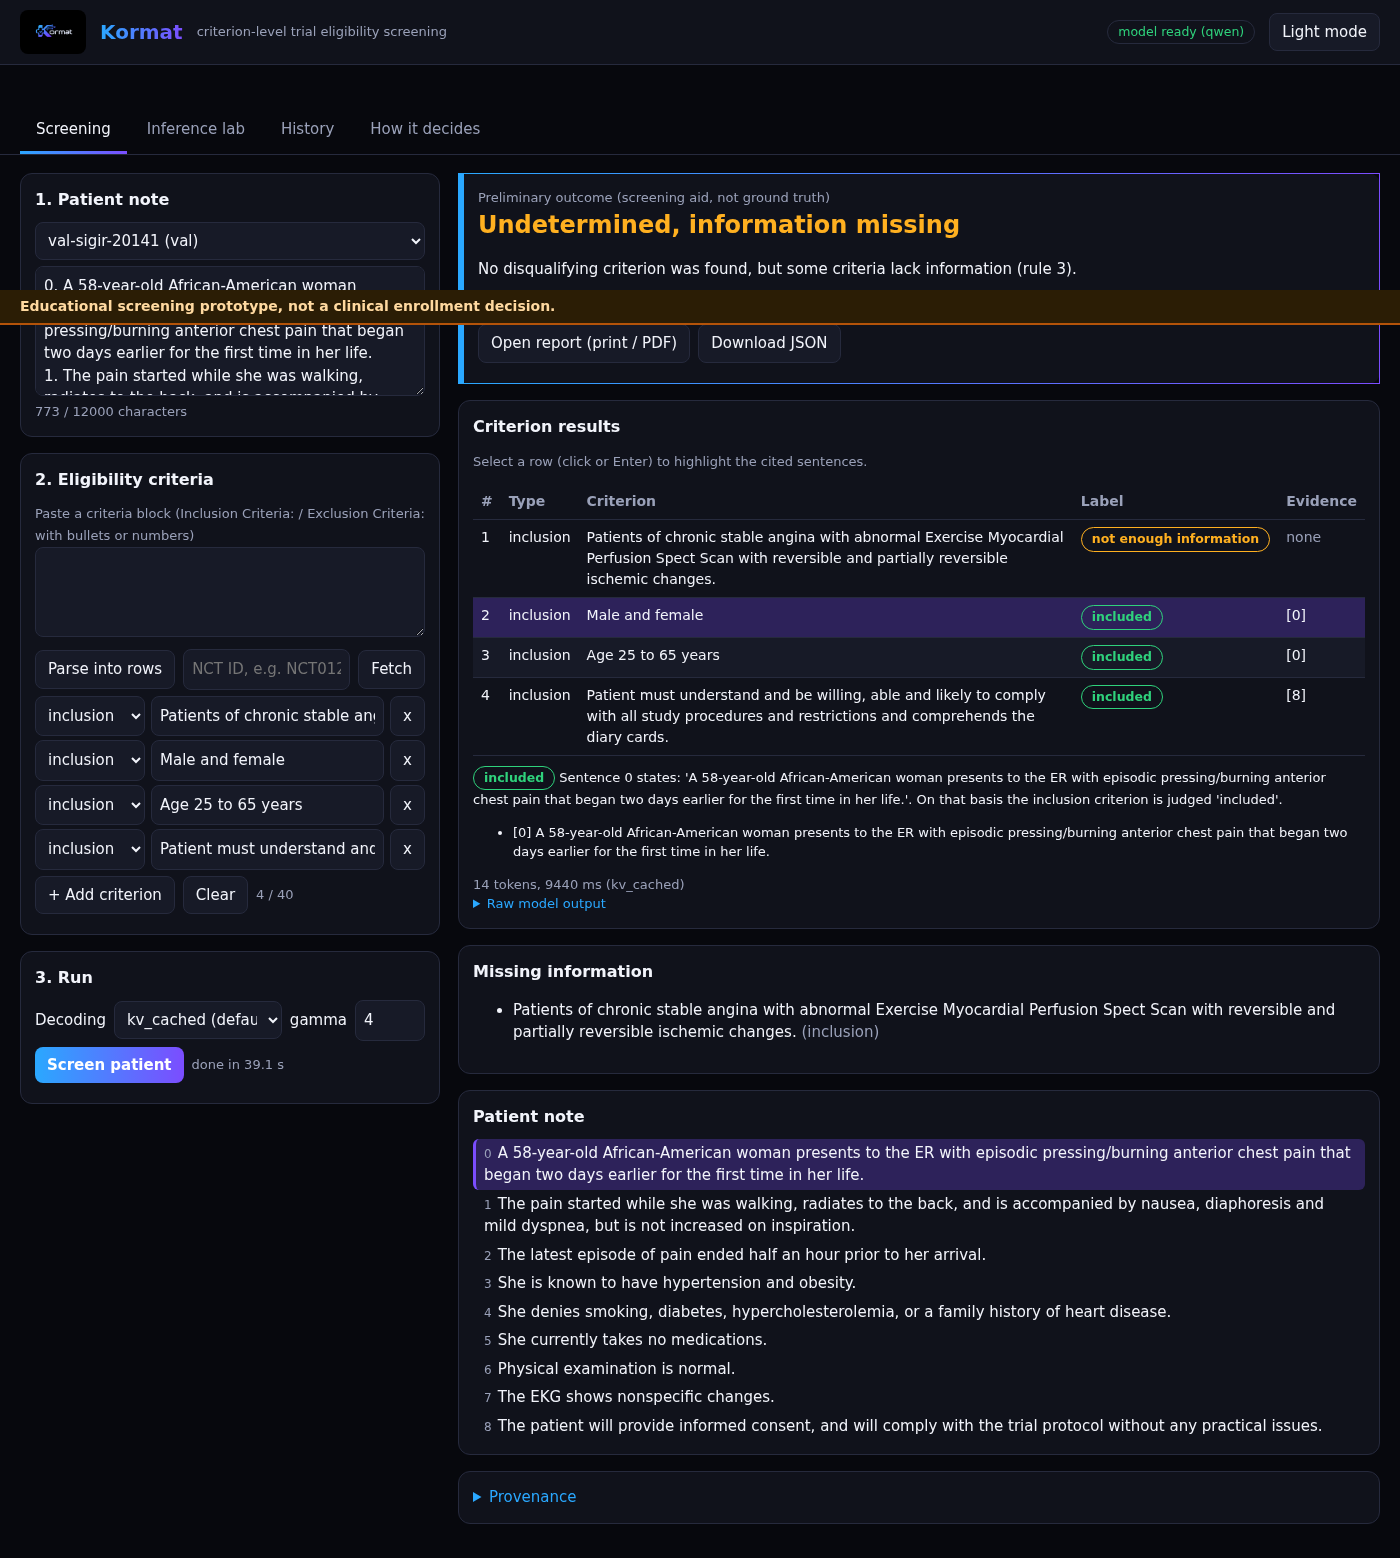
\includegraphics[width=\columnwidth]{figures/app_real_results.png}
\caption{Kormat screening a validation patient with the fine-tuned model (real engine, KV-cached decoding). The second criterion is selected and its cited sentence~0 is highlighted in the numbered note. The missing-information list and the rule-based preliminary outcome are shown, together with the disclaimer banner.}\label{fig:app}
\end{figure}
\begin{figure}[t]\centering
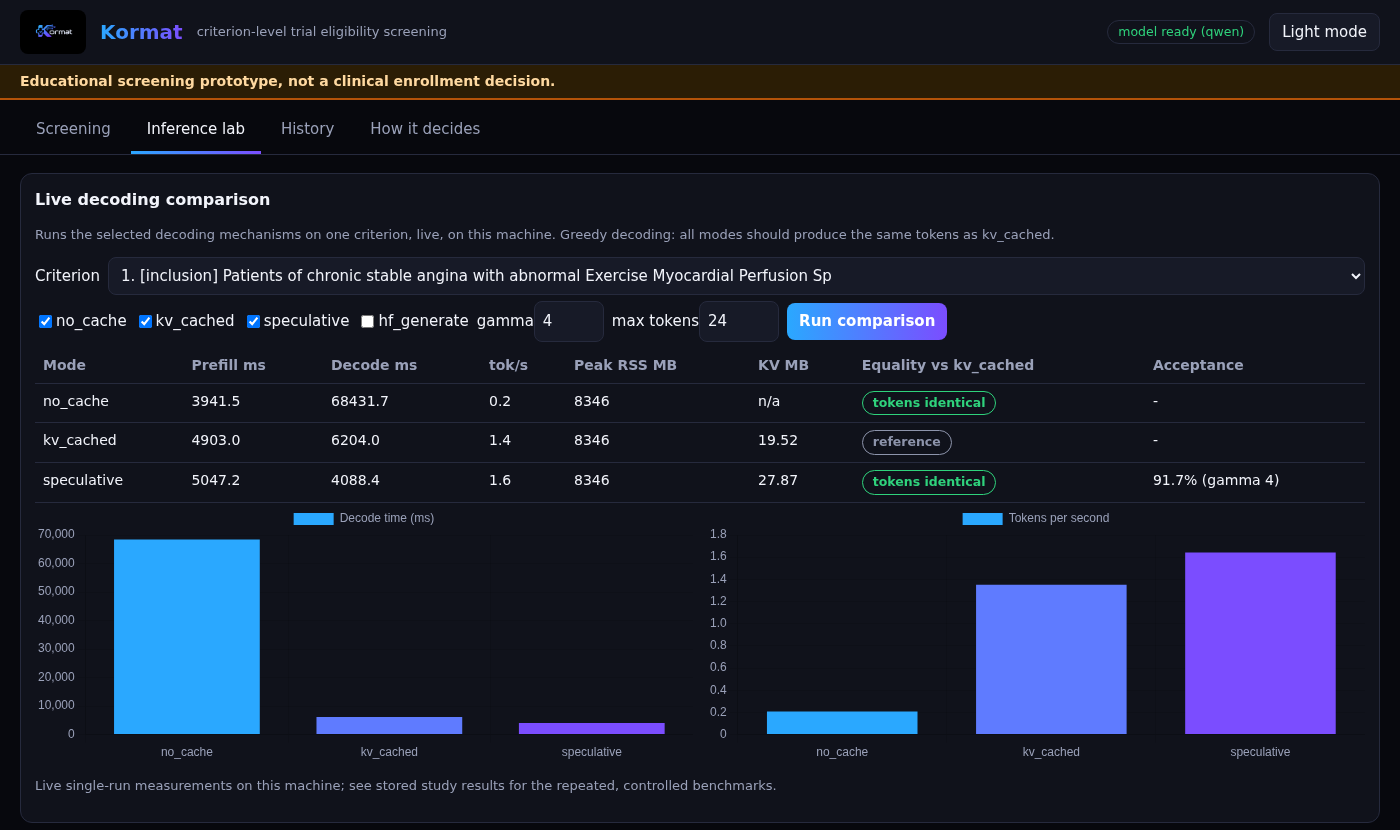
\includegraphics[width=\columnwidth]{figures/app_real_lab.png}
\caption{Inference lab: the same criterion decoded live with no cache, our KV cache and speculative decoding ($\gamma=4$). The lab shows timings, memory, acceptance rate and token equality against the KV-cached reference.}\label{fig:lab}
\end{figure}
Fig.~\ref{fig:app} shows the screening workflow on the real fine-tuned model. A user pastes a note (free text is split into numbered sentences), enters or pastes the criteria (or fetches them by NCT ID), and runs the screen. Each criterion row shows the label, the cited IDs and an explanation quoted only from those sentences, and clicking a row highlights the evidence. In a recorded real-engine session (\texttt{results/app/*/real\_smoke.json}), with the evaluation running concurrently on the same CPU, the model loaded in 15\,s from the local cache. Each criterion took 9.5--10.4\,s, and all four criteria of the sample patient matched the expert labels. The patient--trial outcome is an explicit rule (any exclusion met or inclusion unmet $\Rightarrow$ likely ineligible; otherwise any missing information $\Rightarrow$ undetermined; otherwise potentially eligible). The app presents it as a preliminary aggregation, never as ground truth.

The lab (Fig.~\ref{fig:lab}) re-runs any criterion live under each decoding mode. For a 24-token output, no-cache decoding took 68.9\,s, KV-cached decoding 6.2\,s and speculative decoding 4.0\,s, with an acceptance rate of 91.7\%. All three produced the same tokens, which the lab confirms with an equality badge. On this longer output speculative decoding did help, consistent with the analysis above: the gain appears once decoding, not prefill, dominates. Invalid inputs (empty note, too many criteria, malformed criteria, the model still loading, an offline NCT fetch) return explanatory messages and the app keeps working; the automated tests cover each case. Reports export as print-ready HTML and JSON with provenance (model and adapter revision, adapter hash, git commit, decoding settings) and persist across restarts.
